 %%%%%%%%%%%%%%%%%%%%%%% file template.tex %%%%%%%%%%%%%%%%%%%%%%%%%
%
% This is a general template file for the LaTeX package SVJour3
% for Springer journals.          Springer Heidelberg 2010/09/16
%
% Copy it to a new file with a new name and use it as the basis
% for your article. Delete % signs as needed.
%
% This template includes a few options for different layouts and
% content for various journals. Please consult a previous issue of
% your journal as needed.
%
%%%%%%%%%%%%%%%%%%%%%%%%%%%%%%%%%%%%%%%%%%%%%%%%%%%%%%%%%%%%%%%%%%%
%
% First comes an example EPS file -- just ignore it and
% proceed on the \documentclass line
% your LaTeX will extract the file if required
%\begin{filecontents*}{example.eps}
%!PS-Adobe-3.0 EPSF-3.0
%%BoundingBox: 19 19 221 221
%%CreationDate: Mon Sep 29 1997
%%Creator: programmed by hand (JK)
%%EndComments

%\end{filecontents*}
%
\RequirePackage{fix-cm}
%
\documentclass{svjour3}                     % onecolumn (standard format)
%\documentclass[smallcondensed]{svjour3}     % onecolumn (ditto)
%\documentclass[smallextended]{svjour3}       % onecolumn (second format)
%\documentclass[twocolumn]{svjour3}          % twocolumn
%
\smartqed  % flush right qed marks, e.g. at end of proof
%
\usepackage{graphicx}
\usepackage{natbib}
\renewcommand{\figurename}{Fig.}
\newcommand{\reffig}[1]{Fig. \ref{#1}}
\usepackage{graphicx}
\usepackage{amsmath,amsfonts}
\usepackage{multirow,booktabs}
\usepackage{subfigure}
\usepackage{setspace}
\usepackage{lineno}
\usepackage{color}


%
% \usepackage{mathptmx}      % use Times fonts if available on your TeX system
%
% insert here the call for the packages your document requires
%\usepackage{latexsym}
% etc.
%
% please place your own definitions here and don't use \def but
% \newcommand{}{}
%
% Insert the name of "" with
\journalname{Plant and Soil}


%

\begin{document}
\title{Semi-active control of a structure using magneto-rheological dampers based on the reinforcement learning
%\thanks{Grants or other notes
%about the article that should go on the front page should be
%placed here. General acknowledgments should be placed at the end of the article.}
}

%\titlerunning{Short form of title}        % if too long for running head

\author{Yang Yang$^1$
         %etc.
}

%\authorrunning{Short form of author list} % if too long for running head

\institute{ 
           $*$ Yang Yang  \at
              \email{smiba@qq.com}  
              \and
             1 College of Water Conservancy and Hydropower Engineering, Hohai University, Nanjing 210098, China \\
}

\date{Received: date / Accepted: date}
% The correct dates will be entered by the editor


\maketitle


\begin{abstract}





\keywords{Reinforcement learning; Semi-active; vibration control; MR damper;}
% \PACS{PACS code1 \and PACS code2 \and more}
% \subclass{MSC code1 \and MSC code2 \and more}
\end{abstract}

\section{Introduction}
In this study, we focus on 
\section{The model of motion of structures}
The equation of motion of a controlled building with n degree of freedom subjected to an earthquake load can be expressed as:
\begin{equation}M\ddot{X}(t)+C\dot{X}(t)+KX(t)=-M\Gamma\ddot{x}_g+B_sF(t)\end{equation}\label{1}
where M, C, and K are the $n \times n$  mass, damping, and stiffness matrices of a controlled building. $X(t)$, $\dot{X}(t)$, and $\ddot{X}(t)$ the displacement, velocity, and acceleration with respect to the base.
F(t) is the force produced by the damper. $\ddot{x}_g$ is the acceleration of an earthquake. 

For Equation\ref{1}, the corresponding state space equations can be expressed as:
\begin{equation}\dot{x}=Ax+Bu\end{equation}
\begin{equation}y=Cx+Du\end{equation}

where
\begin{subequations}
\begin{equation}       
A=\left[                 
  \begin{array}{cc}   
   0 & I \\  
   -M^{-1}k_s & -M^{-1}C\\ 
  \end{array}
\right]               
\end{equation}

\begin{equation}       
B=\left[                 
  \begin{array}{cc}   
   0 & 0\\  
   -1 & -M^{-1}\Gamma\\ 
  \end{array}
\right]               
\end{equation}

\begin{equation}       
C=\left[                 
  \begin{array}{cc}   
   I & 0\\  
   0 & I\\ 
   -M^{-1}K_s & -M^{-1}C_d
  \end{array}
\right]               
\end{equation}

\begin{equation}       
D=\left[                 
  \begin{array}{cc}   
   I & 0\\  
   0 & I\\ 
   -M^{-1}K_s & -M^{-1}C_d
  \end{array}
\right]               
\end{equation}

\end{subequations}

\begin{figure}[!h]
\centering
{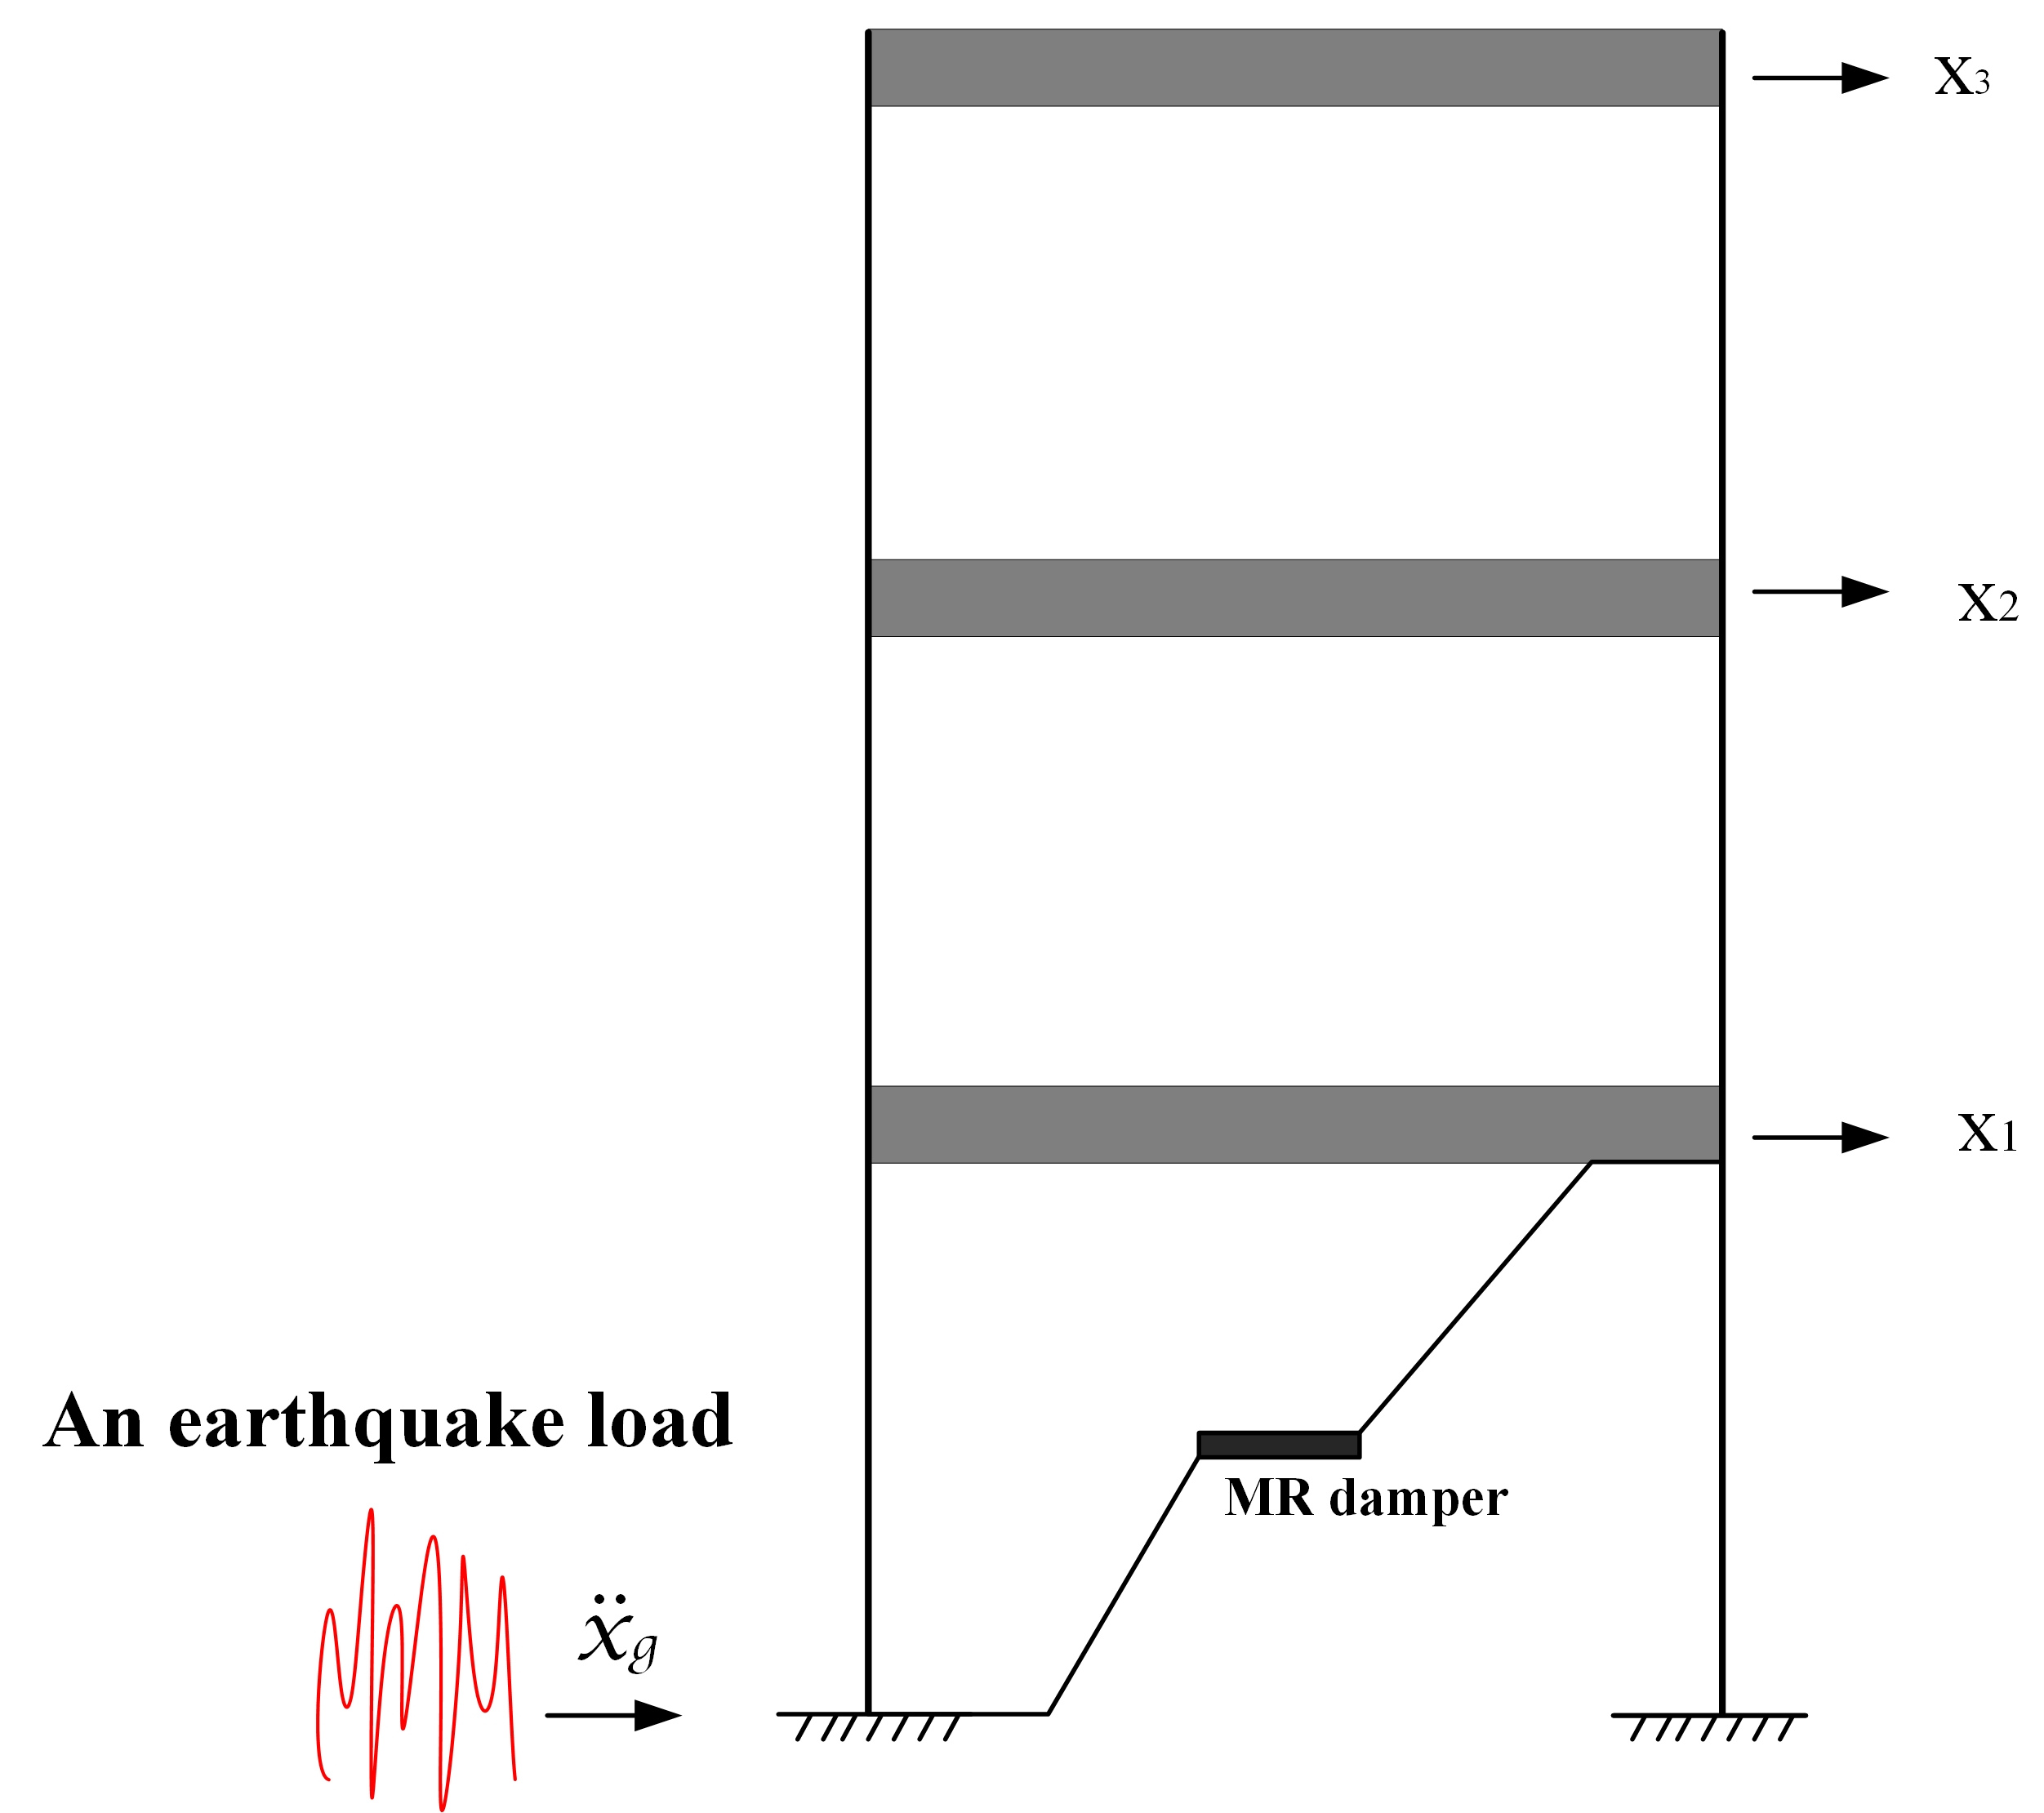
\includegraphics[width=0.6\textwidth]{structure.jpg}} 
\caption{Three-story building with an semi-active control system.} 
\label{structure} 
\end{figure} 

\section{The model of MR damper}


The schematic model is shown in Figure \ref{bouc-wen}

The Bouc-Wen model is written as 
\begin{equation}F=c_0 \dot{x}+k_0(x-x_0)+\alpha z\end{equation}
where $\alpha$ is the Bouc-Wen model parameter related to the MR material yield stress; $k_0$ and $c_0$ are spring stiffness and dashpot damping coefficient respectively. $\dot{z}$ and z are hysteretic deformation of the model which is defined by following equation:
\begin{equation}\dot{z}=-\gamma|\dot{x}|z|z|^{n-1}-\beta \dot{x}|z|^n+A\dot{x}\end{equation}
where $A$, $\beta$, and $\gamma$ are the Bouc-Wen model parameters.

\begin{figure}[!h]
\centering
{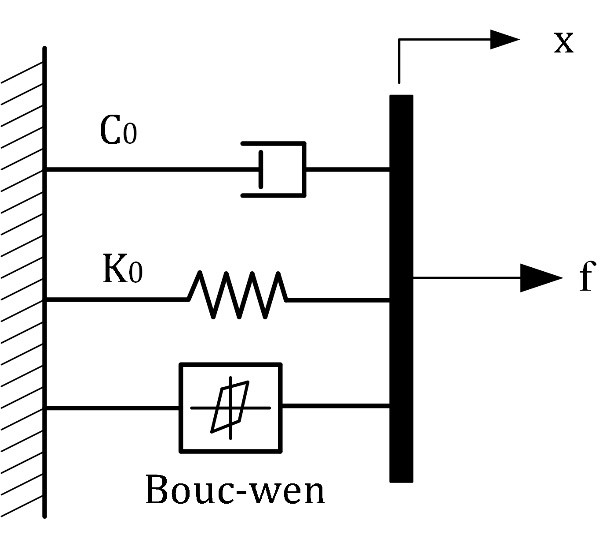
\includegraphics[width=0.6\textwidth]{bouc-wen.jpg}} 
\caption{The schematic diagram of the Bouc-Wen model} 
\label{bouc-wen} 
\end{figure} 

\section{Reinforcement learning control method}

Reinforcement learning is a type of machine learning that can solve sequential decision problems. RL can learn from interaction with an unknown environment to achieve long-term goals \citep{sutton}. The agent-environment interaction in RL is shown in \reffig{interaction}(a). More specifically, the agent and environment interact at each of a sequence of discrete time steps, $t$. The agent observes the state of environment, $s_t \in S$ at each time step, $t$, and then selects an action, $a_t \in A$. After the action selection, the agent obtains a reward $r_{t+1} \in R$, and transits a new state, $s_{t+1}$. 

The goal of agent is to achieve an optimal policy $\pi^*$ that maximize the sum of discounted rewards $G_t$ as follows:
\begin{equation}
G_{t}=R_{t+1}+\gamma R_{t+2}+\gamma^2 R_{t+2}+\cdots=\sum_{k=0}^{\infty} \gamma^{k} R_{t+k+1}
\end{equation}
where $\gamma \in [0,1]$ is called discounted rate, which influences present value of future rewards. 


\begin{equation}Q(S_t,A_t) \leftarrow Q(S_t,A_t)+\alpha [R_{t+1} + \gamma max_{a}Q(S_{t+1,a})-Q(S_t,A_t)]\end{equation}
where $\alpha \in$[0,1] is the learning rate, the ; $\gamma$ $\in$[0,1] is the discount rate. The discount rate determines the present value of future rewards. $A_t$ is the action set. $S_t$ is the state set.


Similarly, controlling MR dampers in the semi-active control can be modeled as a sequential decision problem. 

\begin{figure}[!h]
\centering
{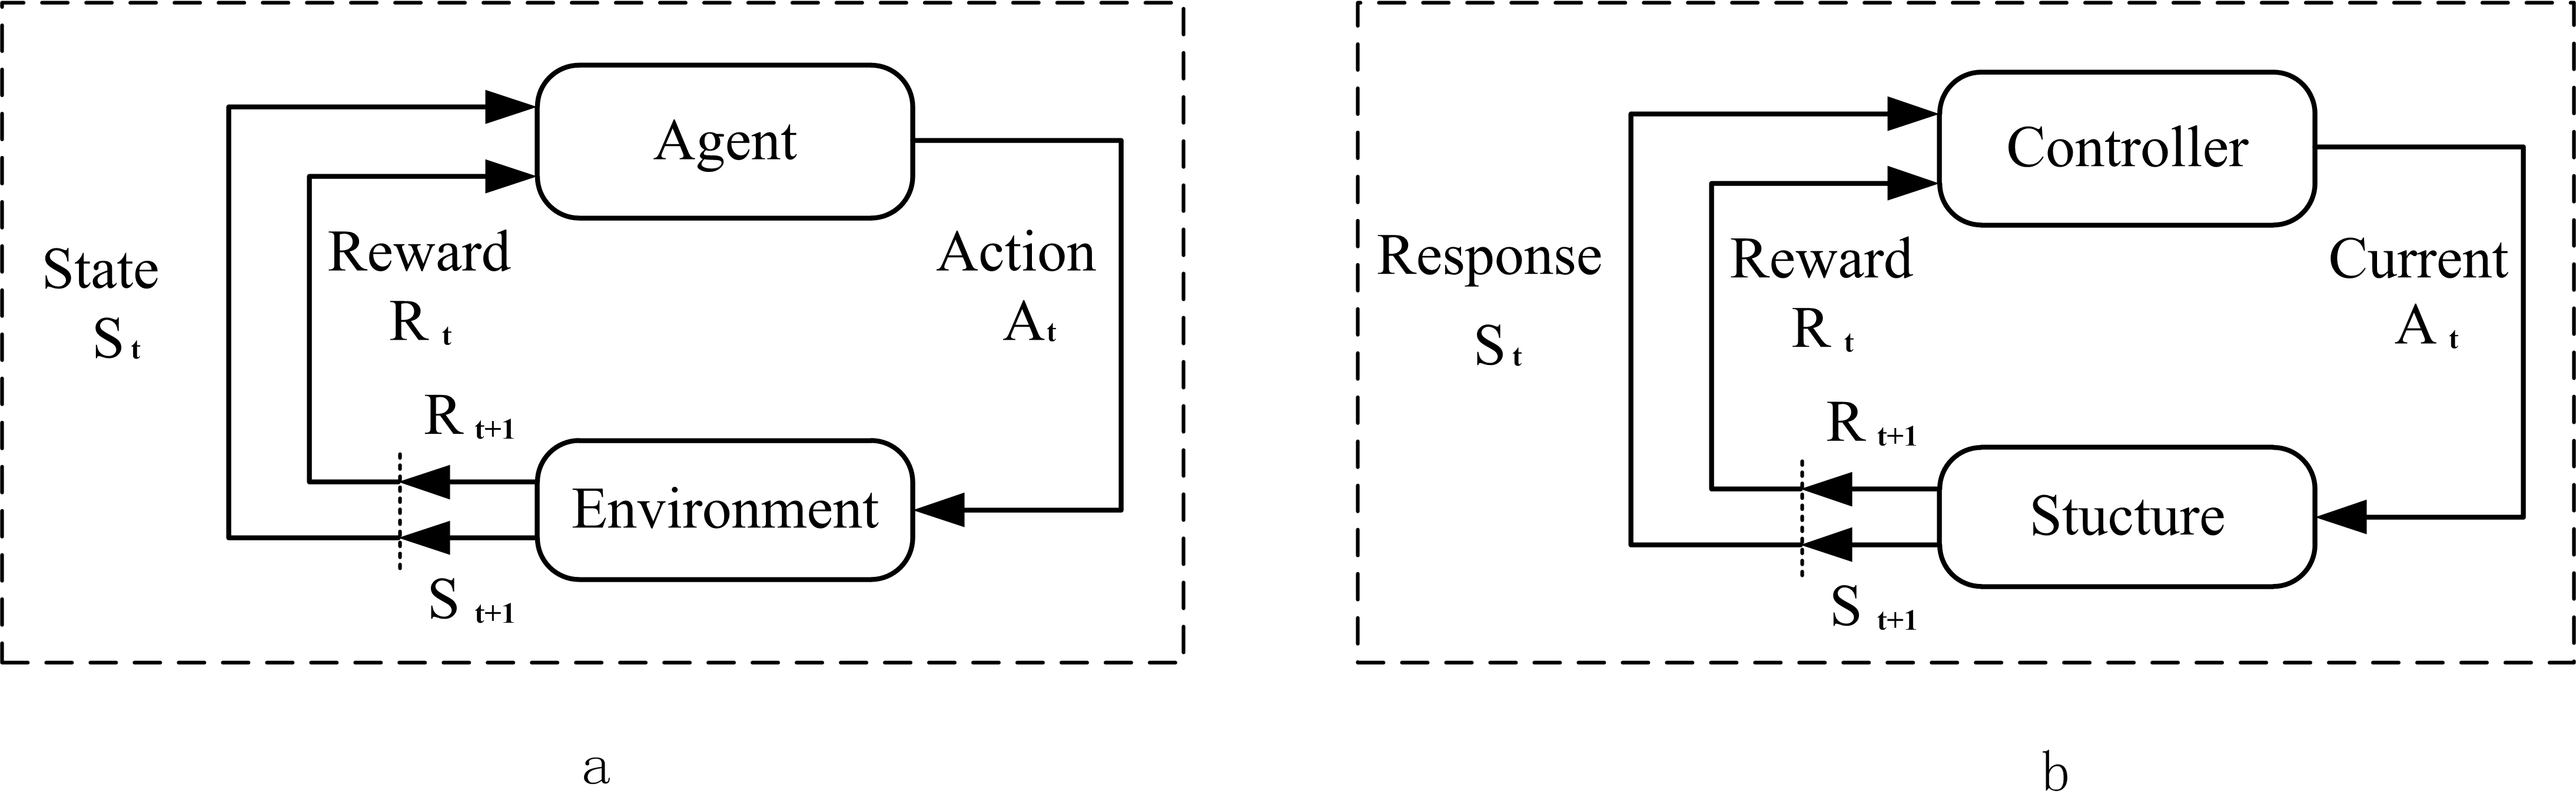
\includegraphics[width=1.0\textwidth]{interaction.jpg}} 
\caption{Agent-environment interaction in reinforcement learning.} 
\label{interaction} 
\end{figure} 
\subsection{Action}

In this study, we control the current $I$ of the MR damper to change its damping force. The maximum working current of MR damper which is used in this study is 1.0 A. Hence, we selected the inputting the current for the MR damper as the actions of an agent $A_i=\{0.1I, 0.2I, 0.3I, 0.4I, 0.5I, 0.6I, 0.7I, 0.8I, 0.9I, 1.0I\}$. 

\subsection{Reward function}


In this study, the reward was defined in

\begin{equation}
R(U_i)=
\begin{cases}
-C \frac{U_{coni}}{U_{unconi}},  & \frac{U_{coni}}{U_{unconi}} > 1 \\
0, & \frac{U_{coni}}{U_{unconi}} = 1 \\
C \frac{U_{unconi}}{U_{coni}}, & \frac{U_{coni}}{U_{unconi}} < 1 
\end{cases}
\end{equation}

where $C$ is a magnification factor of the reward; $U_{coni}$ is the structure response of controlled; $U_{unconi}$ is the structure response of uncontrolled. When $ \frac{U_{coni}}{U_{unconi}} $, the action had not change the structure response. The action had not reduce the structure response, hence, its reward was zero. When $\frac{U_{coni}}{U_{unconi}} > 1$, the action increased the structure response. Hence, its reward (punishment) is $-C \frac{U_{coni}}{U_{unconi}}$. When $\frac{U_{coni}}{U_{unconi}} < 1$, the action decreased the structure response. Hence, its reward is $C \frac{U_{unconi}}{U_{coni}}$. Thus, if an action can reduce more response, it can achieve more reward. In contrary, if an action increased more response, it will obtain more punishment. RL can give its reward according to each action using the reward function. Finally, the optimal action of each step is determined to form the optimal control strategy and realize the optimal control of MR damper.

\subsection{Greedy method}
The agent can select actions by the exploration and exploitation. When agent use the exploration to select actions, it will select the actions of greatest reward.

To balance exploration and exploitation, the researcher proposed a $\epsilon$-greedy method \citep{}. The $\epsilon$-greedy can be written as
\begin{equation}
\pi(a | s)=\left\{\begin{array}{c}
{1-\varepsilon+\frac{\varepsilon}{|A(s)|}, a=\arg \max _{a} Q(s, a)} \\
{\frac{\varepsilon}{|A(s)|}, \quad a \neq \arg \max _{a} Q(s, a)}
\end{array}\right.
\end{equation}

For ,
$a=\arg \max _{a} Q(s, a)$

$1- \epsilon + \frac{\epsilon}{|A(s)|}$
$\frac{\epsilon}{|A(s)|}$

\section{Numerical experiment}
\subsection{Model parameters}
The performance of the proposed reinforcement learning control algorithm was evaluated in one example through numerical simulation. To demonstrate the proposed control algorithm, a three-story building with a single MR damper was considered. The MR damper was installed in the first floor, as shown in \ref{structure}. The mass $M$, dampering $Cs$ and stiffness $Ks$ matrices are as follows:

\begin{equation}       
M=\left[                 
  \begin{array}{ccc}   
   3.456 & 0 & 0 \\  
    0 & 3.456 & 0 \\ 
   0 & 0 &  3.456 \\
  \end{array}
\right]     
\times 10^{5} kg        
\end{equation}

\begin{equation}       
Cs=\left[                 
  \begin{array}{ccc}   
    1.745 & -0.512 & -0.111\\
    -0.512 & 1.634 & -0.623 \\
    -0.111 & -0.623 & 1.122 \\
  \end{array}
\right]     
\times 10^{5} N s/m        
\end{equation}

\begin{equation}       
Ks=\left[                 
  \begin{array}{ccc}   
  2.4 & -1.2 & 0 \\
  -1.2 & 2.4 & -1.2 \\
  0 & -1.2 & 1.2 \\
  \end{array}
\right]     
\times 10^{8} N/m        
\end{equation}

\subsection{Numerical implementation}
\begin{equation}
R=\left[\begin{array}{ccc}
{r_{11}} & {\cdots} & {r_{1 n}} \\
{\vdots} & {\ddots} & {\vdots} \\
{r_{m 1}} & {\cdots} & {r_{m n}}
\end{array}\right]
\end{equation}
where $r_{mn}$ is the reward of each action, $m$ is the number of the state, $n$ is the number of the action. 

\begin{equation}
\mathrm{Q}=\left[\begin{array}{ccc}
{q_{11}} & {\cdots} & {q_{1 n}} \\
{\vdots} & {\ddots} & {\vdots} \\
{q_{m 1}} & {\cdots} & {q_{m n}}
\end{array}\right]
\end{equation}

where $q_{mn}$ is the 



\section{Results and Discussions}
\subsection{The effect of reward function}
\subsection{The effect of RL parameters}
\subsection{The effect of semi-active control by RL}
\section{Conclusions}





% BibTeX users please use one of
\bibliographystyle{spbasic}      % basic style, author-year citations
%\bibliographystyle{spmpsci}      % mathematics and physical sciences
%\bibliographystyle{spphys}       % APS-like style for physics
%\bibliographystyle{model4-names}
\bibliography{mybibfile}   % name your BibTeX data base

% Non-BibTeX users please use
%\begin{thebibliography}{}
%
% and use \bibitem to create references. Consult the Instructions
% for authors for reference list style.
%

% etc

\end{document}

% end of file template.tex